\documentclass[letterpaper,12pt]{article}
\usepackage{courier}
\usepackage{fancyheadings}
\usepackage{verbatim}
\usepackage{hyperref}
\usepackage{graphicx}
\pagestyle{fancy}
\setlength\textwidth{6.5in}
\setlength\textheight{8.5in}
\newtheorem{problem_statement}{Problem Statement}
\newcommand{\TBC}{\framebox{\textbf{TO BE COMPLETED}}}
\newtheorem{assumption}{Assumption}
\newcommand{\be}{\begin{enumerate}}
\newcommand{\ee}{\end{enumerate}}
\newcommand{\bi}{\begin{itemize}}
\newcommand{\ei}{\end{itemize}}
\newtheorem{notation}{Notation}
\newtheorem{definition}{Definition}
\newcommand{\ReportDate}{Jan 1, 2023}
\newcommand{\NumDataSets}{42}
\newcommand{\NumFormulas}{5}

\newcommand{\NumPLPSuccessA}{42}
\newcommand{\NumPLPErrorsA}{0}
\newcommand{\AvgTimePLPA}{1.234}

\newcommand{\NumPLPErrorsB}{0}
\newcommand{\AvgTimePLPB}{1.234}

\newcommand{\NumDataSetsForModel}{X}
\newcommand{\NumModelsAttempted}{X}
\newcommand{\NumModelsSucceeded}{X}
\newcommand{\ModelMinTime}{X}
\newcommand{\ModelMaxTime}{X}
\newcommand{\ModelAvgTime}{X}

\begin{document}
\title{Overview of DFE Run}
\author{Automated}
\maketitle
\thispagestyle{fancy}
\lhead{}
\chead{}
\rhead{}
% \lfoot{{\small Decision Sciences Team}}
\cfoot{}
\rfoot{{\small \thepage}}

\begin{abstract}
\ This is an automatically generated report. It is meant ot illustrate the kinds
of analysis that can be performed in LightR.
\end{abstract}

\section{Overview}

\bi
\item The report was generated on \ReportDate. 
\item The number of data sets was \NumDataSets.
\item The number of formulas per model was \NumFormulas.
  \ei

\section{Basic Feature Engineering}
\label{PLP1}
\bi
\item The number of times this was invoked was \NumDataSets
\item The number of errors reported during the first round of feature
  engineering was \NumPLPErrorsA.
\item The average time taken was \AvgTimePLPA
\ei

Distribution of error codes is shown in Table~\ref{plp1_errs}
\begin{table}
  \centering
  \begin{tabular}{|l|l|} \hline \hline
    {\bf Error Code} & {\bf Number} \\ \hline 
    \input{plp1_error_codes.csv} 
    \hline
  \end{tabular}
  \caption{Error Counts for basic feature engineering}
  \label{plp1_errs}
\end{table}

\section{Formula Specific Feature Engineering}
\label{PLP2}

\bi
\item The number of times this was invoked was \NumPLPSuccessA
\item The number of data sets that had at least one error was
  \NumPLPErrorsB.
\item The average time taken was \AvgTimePLPB
\ei

Distribution of error codes is shown in Table~\ref{plp2_errs}
\begin{table}
  \centering
  \begin{tabular}{|l|l|l|} \hline \hline
    {\bf Formula} & {\bf Error Code} & {\bf Number} \\ \hline 
    \input{plp2_error_codes.csv} 
    \hline
  \end{tabular}
  \caption{Error Counts, broken down by formula}
  \label{plp2_errs}
\end{table}

\section{Model Building}
\bi
\item The number of data sets for which model building was attempted was
  \NumDataSetsForModel
\item The number of models attempted was \NumModelsAttempted
\item The number of models that were built was \NumModelsSucceeded
\item Summary statistics of time (in seconds) to build a model
  \bi
\item Minimum \ModelMinTime
\item Maximum \ModelMaxTime
\item Average \ModelAvgTime
\ei
\item Distribution of build times is in Figure~\ref{fig_model_build_times}
\ei
\begin{figure}
\fbox{
  \begin{minipage}{6.0in}
  \centering
  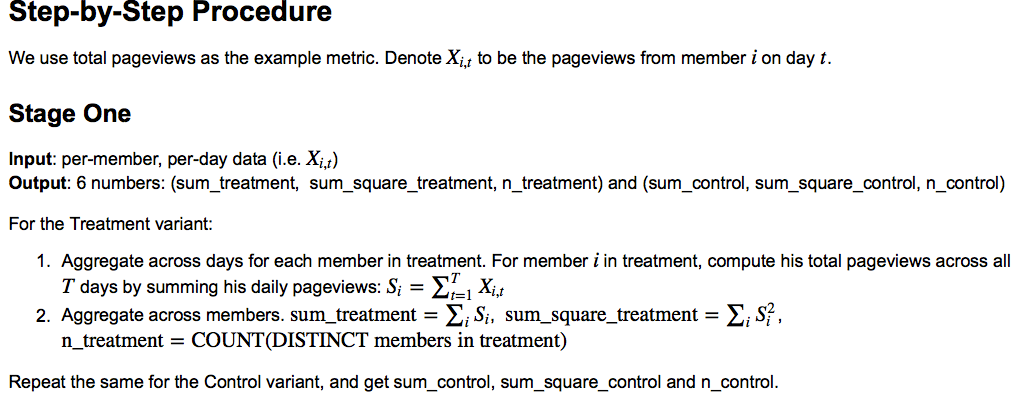
\includegraphics[width=4.5in]{model_build_times.png}
    \caption{Distribution of model build times (seconds)}
  \label{fig_model_build_times}
  \end{minipage}
}
\end{figure}

\section{Error Codes}

\subsection{Basic Feature Engineering}
See Table~\ref{explanation_plp1_errs}
\begin{table}
  \centering
  \begin{tabular}{|l|l|} \hline \hline
    {\bf Error Code} & {\bf Explanation} \\ \hline 
    0 & No Error \\ \hline 
    \hline
  \end{tabular}
  \label{explanation_plp1_errs}
  \caption{Explanation of Error Codes}
\end{table}

\subsection{Formula Specific Feature Engineering}

See Table~\ref{explanation_plp2_errs}
\begin{table}
  \centering
  \begin{tabular}{|l|l|} \hline \hline
    {\bf Error Code} & {\bf Explanation} \\ \hline 
    0 & No Error \\ \hline 
    \hline
  \end{tabular}
  \label{explanation_plp2_errs}
  \caption{Explanation of Error Codes}
\end{table}

\end{document}

